% -----------------------------------------------------------------------------
\section{Openquake demos}
%
OpenQuake usage help can be obtained by simply typing
\begin{Verbatim}[frame=single, commandchars=\\\{\}, fontsize=\small]
openquake@ubuntu:/media/vbox$ openquake 
\end{Verbatim}
and pressing \texttt{<ENTER>}. The provided info will be 
\begin{Verbatim}[frame=single, commandchars=\\\{\}, fontsize=\small]
usage: openquake [-h] [--version] [--force-inputs] [--config-file CONFIG_FILE]
                 [--output-type {db,xml}]
                 [--log-level {debug,info,warn,error,critical}]
                 [--log-file LOG_FILE] [--list-calculations]
                 [--list-outputs CALCULATION_ID]
                 [--export OUTPUT_ID TARGET_DIR] 
\end{Verbatim}
The main execution of OpenQuake is undertaken via the following 
command-line instruction (note that from this point on we'll indicate the 
the command prompt with a simple \texttt{\$}.

An OpenQuake analysis can be launched with the following command
\begin{Verbatim}[frame=single, commandchars=\\\{\}, fontsize=\small]
$ openquake --\textcolor{red}{config_file}=/PATH/TO/CONFIG/FILE --\textcolor{red}{output_type}=xml
\end{Verbatim}
%
\clearpage
\subsection{I exercise: Peer test Set 1 Test 10}
% ..............................................................................
% . . . . . . . . . . . . . . . . . . . . . . . . . . . . . . . . . . . > Figure
\begin{figure}[!ht]
\begin{center}
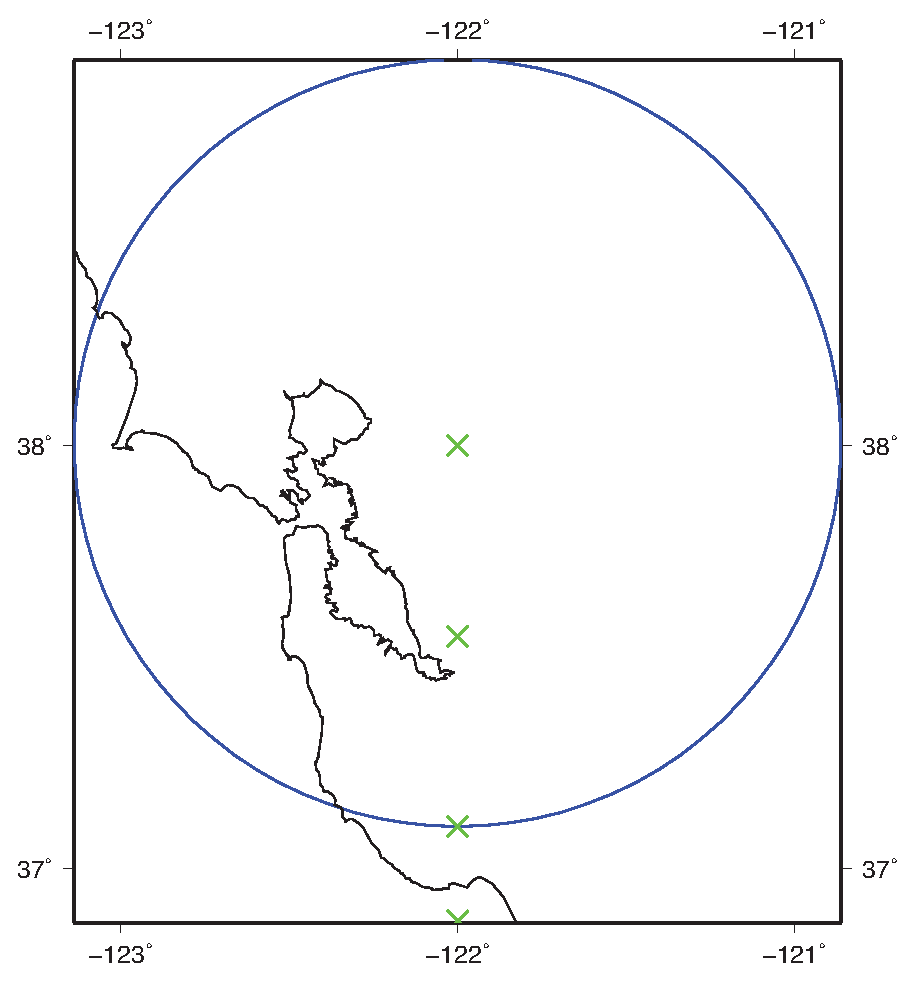
\includegraphics[width=10cm]{./figures/peer_set1_test10/peerSet1test10a.eps}
\caption{PEER Set 1 Test 10: area source geometry and position of sites (green
    crosses)}
\label{fig:demo_peer_set1_test10}
\end{center}
\end{figure}
% . . . . . . . . . . . . . . . . . . . . . . . . . . . . . . . . . . . < Figure
% ..............................................................................
%
For the user with a local installation of OpenQuake, the input files for 
this demostration can be found in the subfolder \texttt{PeerTestSet1Case10} 
in the \texttt{/media/vbox/demos/} directory \marginpar{What about OATS users?}

The first demonstration consists of a simple input model included in the 
PSHA test calculations proposed by \citet{thomas2010}.

The input model consists of one circular area source as it is 
represented in \ref{fig:demo_peer_set1_test10}; the radius of the source 
is sligthly more than one degree of longitude (at 38 degrees latitude) 
which corresponds to about 88km.

Let's move to our root folder \texttt{/media/vbox} and launch
the analysis using the command:
\begin{Verbatim}[frame=single, commandchars=\\\{\}, fontsize=\small]
$ openquake --config_file=./demos/PeerTestSet1Case10/config.gem --output_type=xml
\end{Verbatim}
The calculation should be completed in about one minute. Once completed
in the \texttt{/media/\-vbox/\-demos/\-PeerTestSet1Case10} there'll be a new
folder called \texttt{computed\_results} containing the computed products.
In particular, we'll find two files named \texttt{hazardcurve-0.xml} and
\texttt{hazardcurve-mean.xml}.

Figure \ref{fig:demo_peer_set1_test10_hc} shows the hazard curves computed 
in the four reference points established for this test. 
The hazard curves shows the probability of exceedance in a 
period of one year for a set of PGA values. 
Moving from the southermost point (point A) to the one located at the 
center of the circular area (point D) the hazard clearly tends to increase.
This is justified by the fact that the more a site approaches the center
the higher are the contributions coming from the different sectors of the 
area source.

To better understand from a quantitive point of view these thoughts 
we'll perform later a disaggregation analysis for some hazard values 
computed in the different reference sites.
% ..............................................................................
% . . . . . . . . . . . . . . . . . . . . . . . . . . . . . . . . . . . > Figure
\begin{figure}[ht]
\centering
    \begin{subfigure}[t]{0.4\textwidth}
        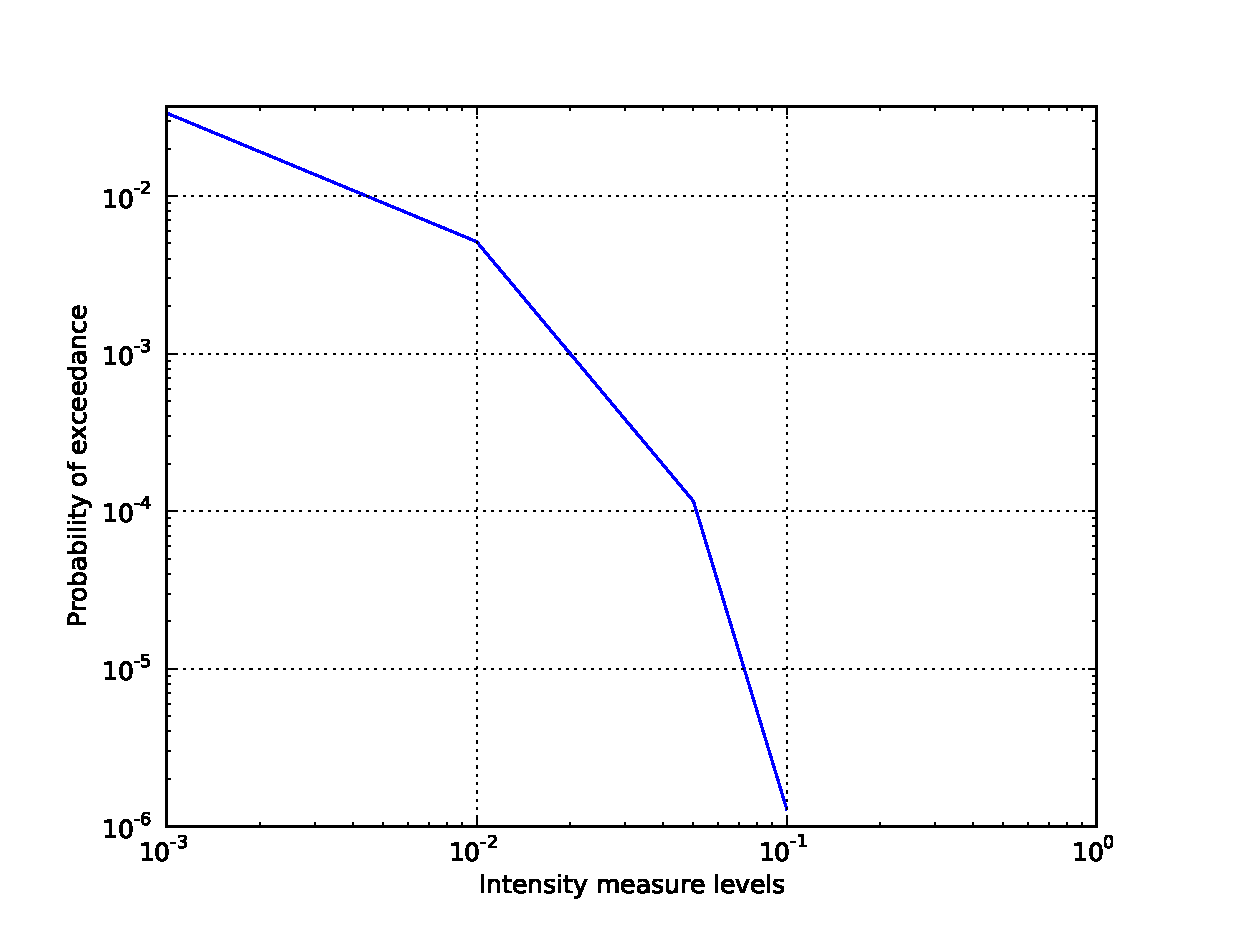
\includegraphics[width=\textwidth]{./figures/peer_set1_test10/000_-122.00_36.87.eps}
        \caption{Site A}
    \end{subfigure}
    \begin{subfigure}[t]{0.4\textwidth}
        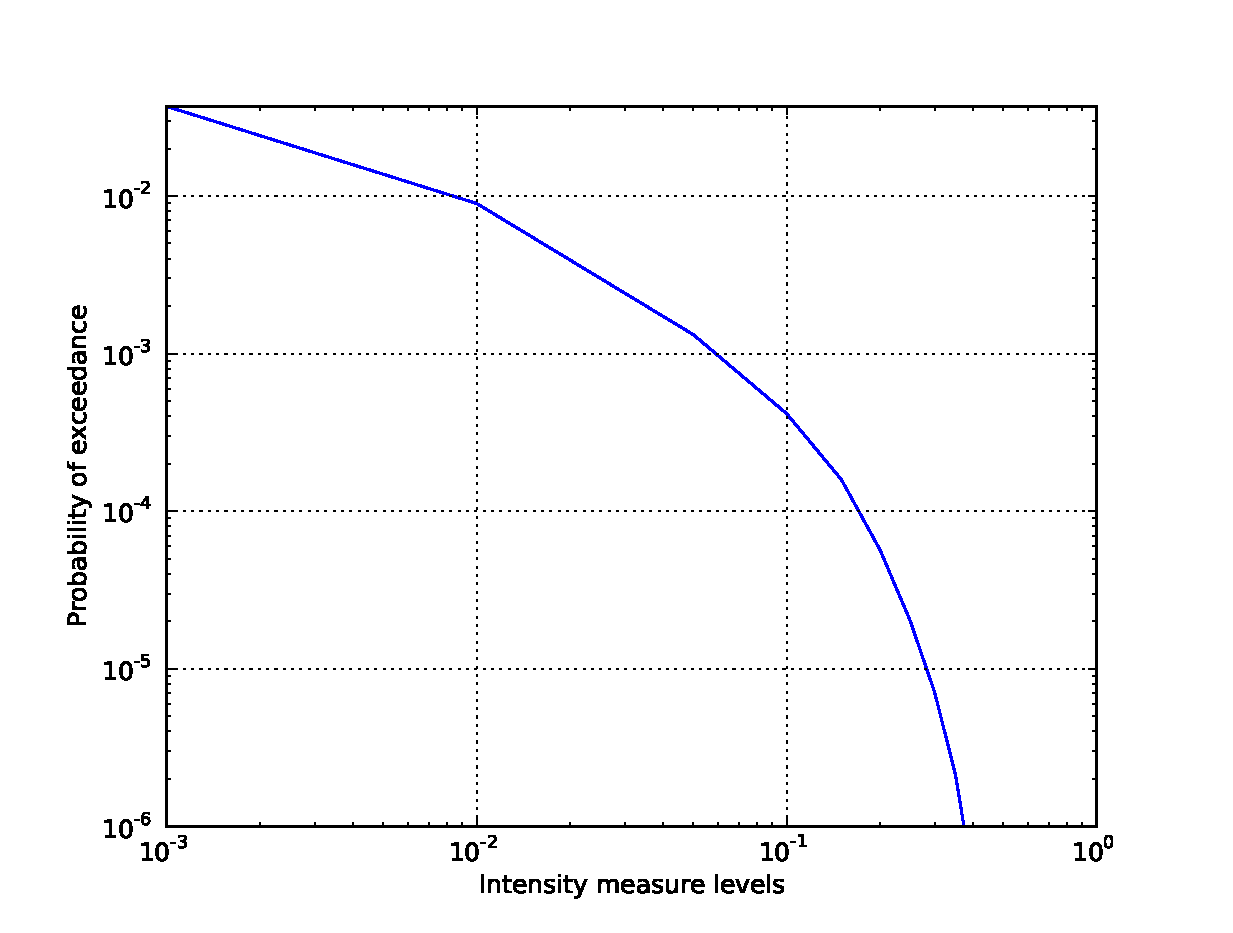
\includegraphics[width=\textwidth]{./figures/peer_set1_test10/001_-122.00_37.10.eps}
        \caption{Site B}
    \end{subfigure}
    \begin{subfigure}[b]{0.4\textwidth}
        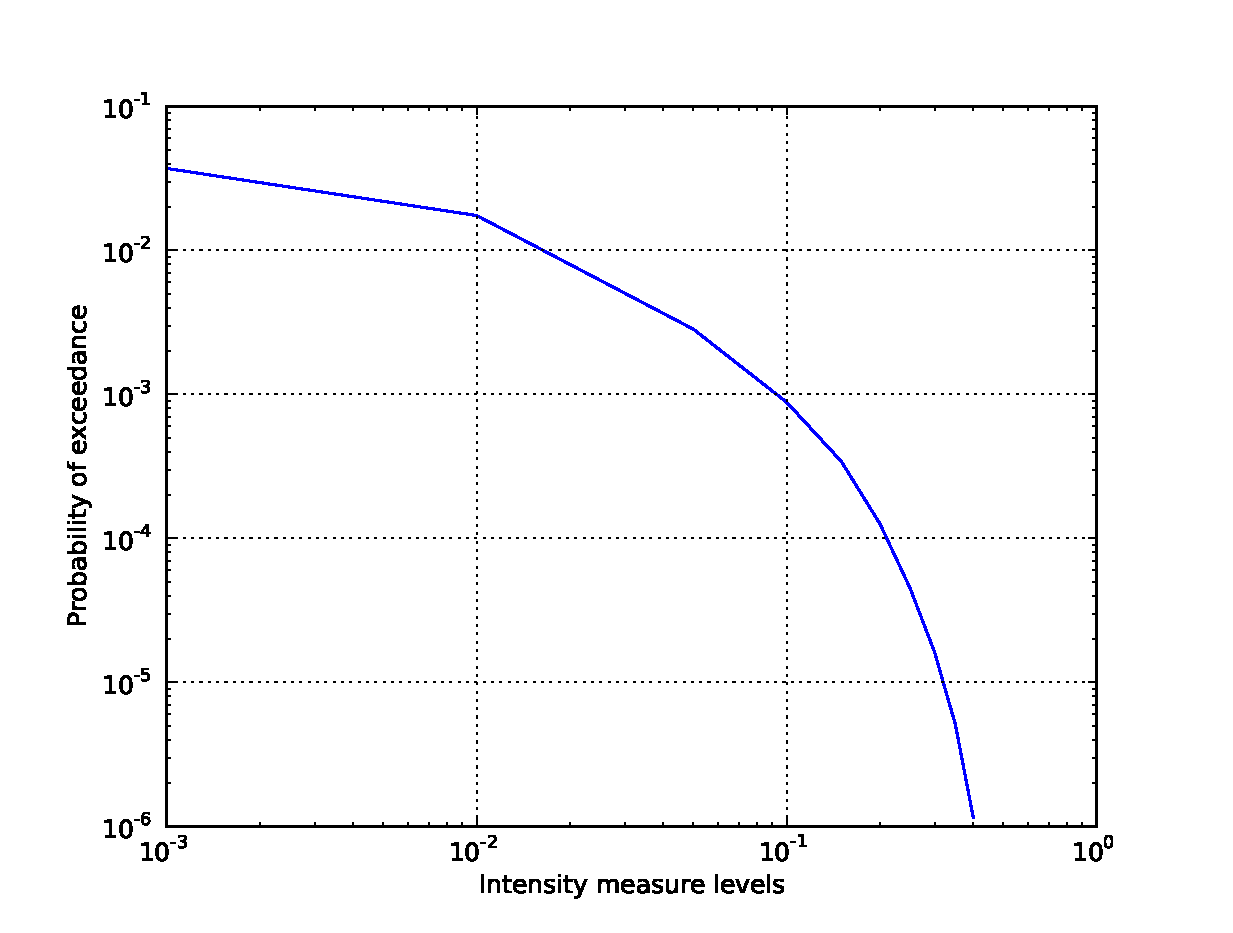
\includegraphics[width=\textwidth]{./figures/peer_set1_test10/003_-122.00_37.55.eps}
        \caption{Site C}
    \end{subfigure}
    \begin{subfigure}[b]{0.4\textwidth}
        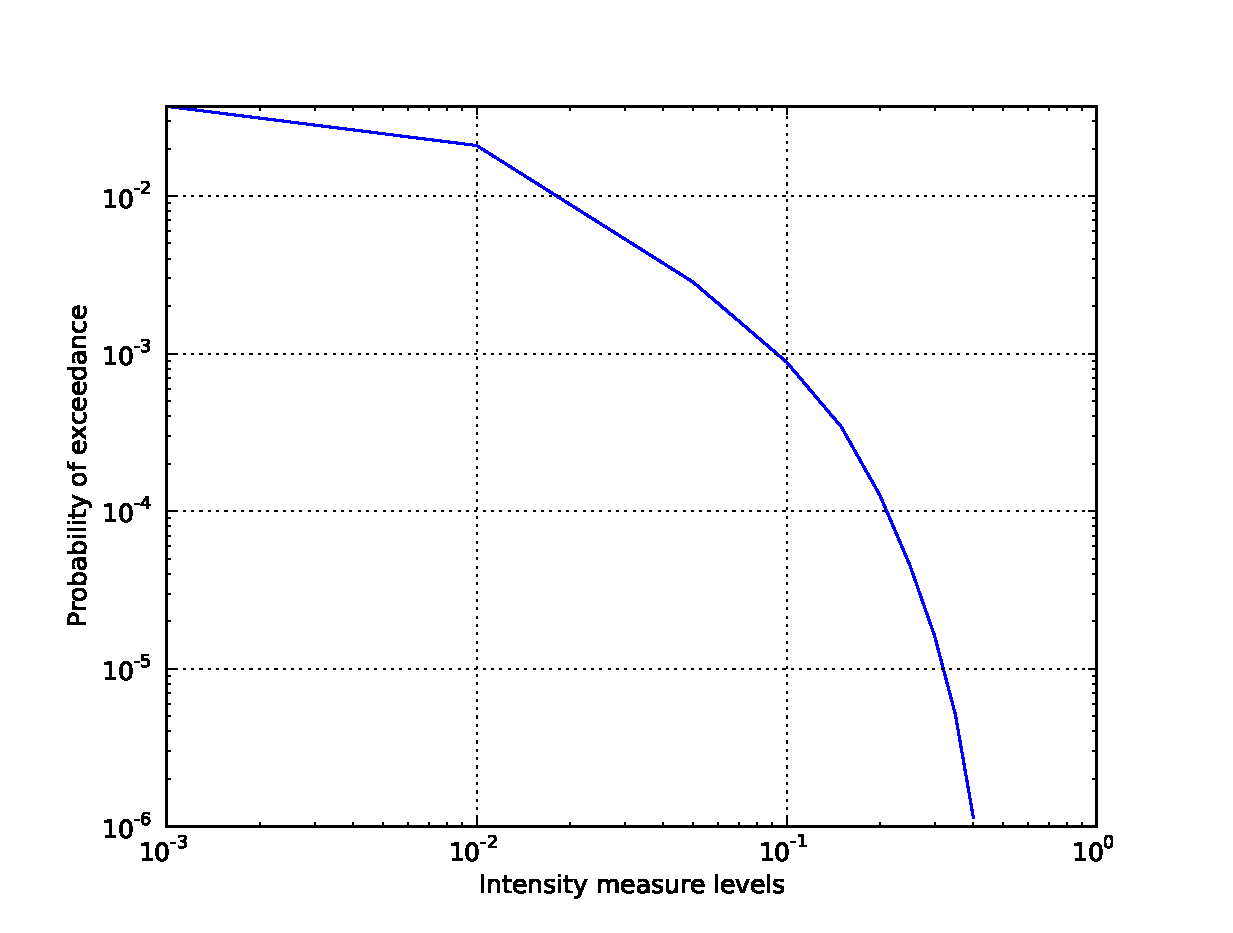
\includegraphics[width=\textwidth]{./figures/peer_set1_test10/002_-122.00_38.00.eps}
        \caption{Site D}
    \end{subfigure}
\caption{PEER Set 1 Test 10: hazard curves in the four sites considered}
\label{fig:demo_peer_set1_test10_hc}
\end{figure}
% . . . . . . . . . . . . . . . . . . . . . . . . . . . . . . . . . . . < Figure
% ..............................................................................
\clearpage
\subsection{II exercise: Area source demo hazard}
%
The input files for this demostration can be found in the folder 
\texttt{area\_\-source\_\-demo\_\-hazard}

The input information consists of a PSHA input model for South East Asia 
developed in the context of the GSHAP project. This input model contains 
xx area sources covering China, India, Mongolia and xxx peninsula.

% ..............................................................................
% . . . . . . . . . . . . . . . . . . . . . . . . . . . . . . . . . . . > Figure
\begin{figure}[!ht]
\centering
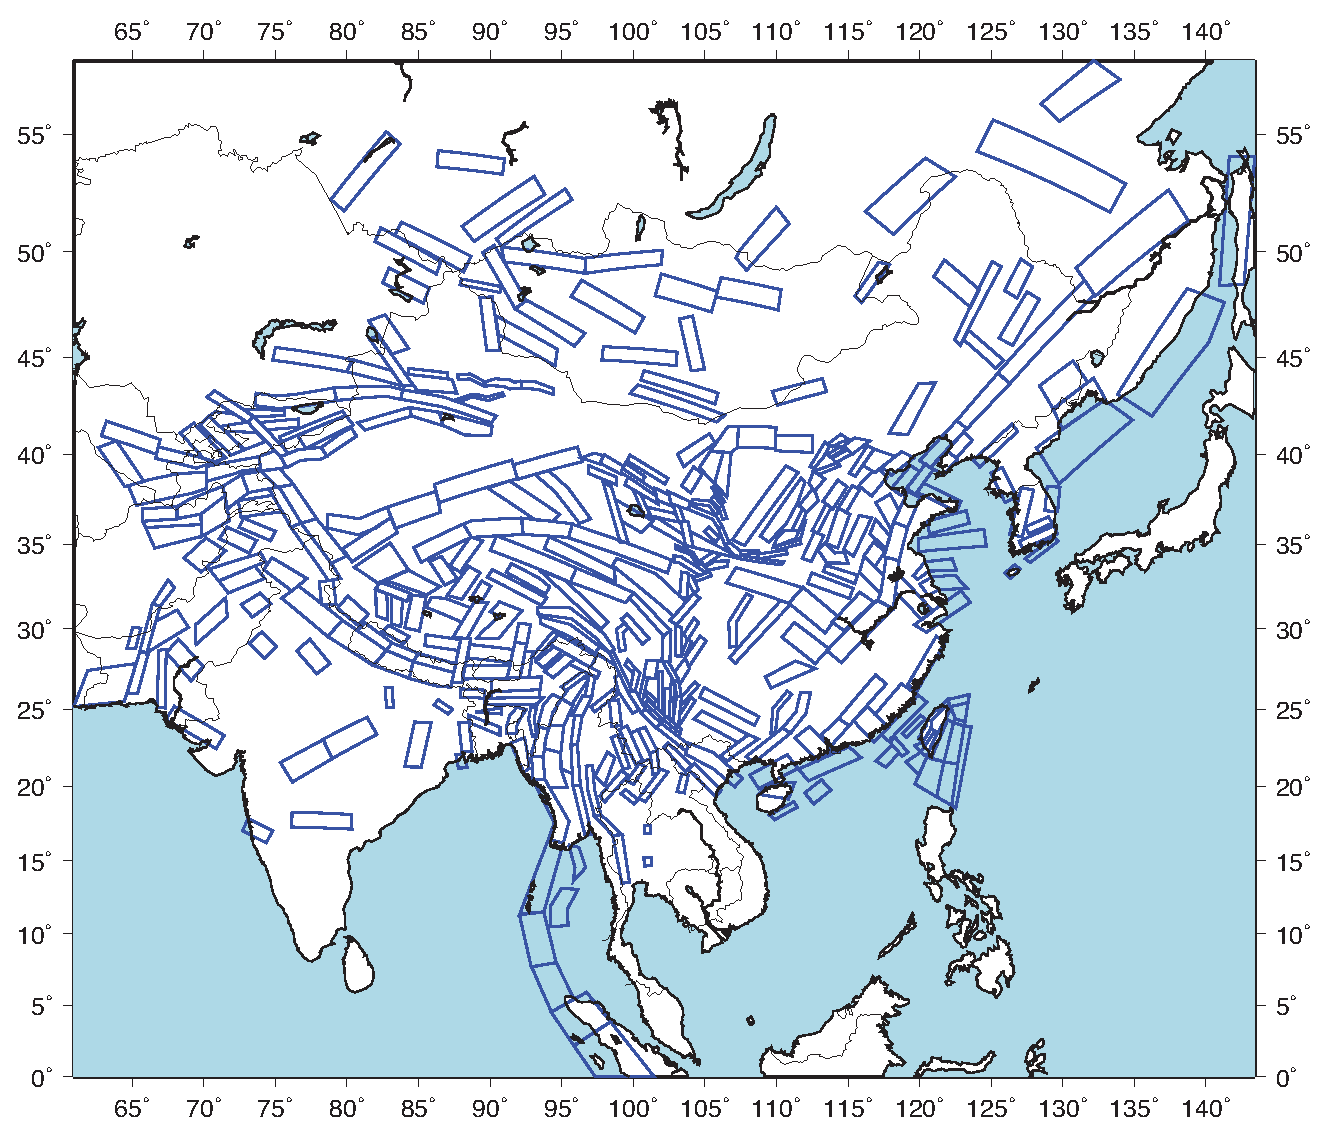
\includegraphics[width=\textwidth,angle=0]{./figures/seAsiaGSHAP.eps}
\caption{South East Asia model developed in the framework of the GSHAP 
project.}
\label{fig:sea_psha_gshap}
\end{figure}
% . . . . . . . . . . . . . . . . . . . . . . . . . . . . . . . . . . . < Figure
% ..............................................................................


\cleardoublepage
